% ===========================================================================
% WORKSHOP VERSION -- 4 pages of content.
%
% This is not an abridgement written by hand. Every equation, proposition,
% theorem and number below is \input from paper/sections/, the same files the
% 9-page paper uses, so the two cannot disagree about the mathematics or the
% results. What is written here rather than shared is the connecting prose,
% which is genuinely different at this length: the paper develops a ladder of
% four rungs, and the workshop states the two that carry the claim.
%
% What is deliberately NOT here, and lives only in the paper:
%   - the discretisation-control experiment (truncation vs quadrature)
%   - Rung 1's gradient-ascent-against-EM comparison
%   - the convergence-rate asymmetry and its stopping rule
%   - the related-work survey, reduced here to the three papers that frame it
%
%   tectonic -X compile workshop.tex
% ===========================================================================
\documentclass{article}

\usepackage[final,nonatbib]{neurips_2023}
\makeatletter\renewcommand{\@noticestring}{}\makeatother
\usepackage[utf8]{inputenc}
\usepackage[T1]{fontenc}
\usepackage{url}
\usepackage{booktabs}
\usepackage{array}
\usepackage{amsfonts}
\usepackage{amsmath}
\usepackage{amssymb}
\usepackage{amsthm}
\usepackage{microtype}
\usepackage{graphicx}
\usepackage[numbers,sort&compress]{natbib}
\usepackage{xcolor}
\usepackage{hyperref}
\definecolor{linknavy}{RGB}{20,60,130}
\definecolor{citegreen}{RGB}{20,100,60}
\hypersetup{colorlinks=true, linkcolor=linknavy, citecolor=citegreen,
            urlcolor=linknavy, filecolor=linknavy}

\renewcommand{\topfraction}{0.9}
\renewcommand{\textfraction}{0.07}
\renewcommand{\floatpagefraction}{0.75}

\graphicspath{{figures/}}
% ===========================================================================
% Shared notation for the internal note and the compendium.
%
% Conventions follow the statistical-physics usage of the diffusion literature
% (Song et al. 2021 for the SDE formulation; Mezard-Montanari 2009 for the
% graphical-model side). Only publicly available sources are cited.
%
% Symbol decisions that matter, fixed here once:
%
%   1. K (or K_theta) is the MARKOV TRANSITION KERNEL, everywhere and only.
%      The number of quadrature grid points is N_g. These were previously W and
%      K respectively, which collided; nothing in either document may now use
%      K for a grid size or W for a kernel.
%
%   2. The chain length is L, and every graphical-model statement is indexed by
%      sites. The ambient dimension equals it, n = L, but the two are written
%      separately because they are different concepts and the reader should not
%      have to infer the identification. The number of observed sequences is M.
%      A translation sentence appears at first use, because much of the
%      diffusion literature uses n for the sample count and d for the dimension.
%
%   5. Vectors are bold lowercase (\vect) and matrices and tensors are bold
%      uppercase (\mat). Scalars, including single sites a_i, stay upright.
%      Anything indexed down to a scalar loses its bold.
%
%   3. The decay factor is written e^{-t} in displayed equations and is never
%      abbreviated to alpha_t.
%
%   4. Gaussian white noise eta is STANDARDISED, <eta(t)eta(t')> = delta(t-t'),
%      so the sqrt(2) is carried explicitly in both the forward and the reverse
%      SDE. This keeps Delta_t = 1 - e^{-2t} consistent throughout.
% ===========================================================================

% --- Diffusion -------------------------------------------------------------
\newcommand{\Pz}{P_0}                       % clean distribution
\newcommand{\Pt}{P_t}                       % noised distribution at time t
\newcommand{\Dt}{\Delta_t}                  % 1 - e^{-2t}
\newcommand{\score}{S}                      % S(x,t) = grad log P_t(x)
\newcommand{\gwn}{\vect{\eta}}              % standardised Gaussian white noise (vector)
\newcommand{\tmin}{t_{\min}}
\newcommand{\tmax}{t_{\max}}

% Posterior mean, in bracket notation rather than E[a|x].
\newcommand{\pmean}[1]{\langle #1 \rangle_{x,t}}
\newcommand{\pmeansite}[1]{\langle a_{#1} \rangle_{x,t}}

% --- Vectors and matrices --------------------------------------------------
% Bold lowercase for vectors, bold uppercase for matrices and tensors.
\newcommand{\vect}[1]{\mathbf{#1}}
\newcommand{\mat}[1]{\mathbf{#1}}
\newcommand{\va}{\vect{a}}                  % clean chain, in R^L
\newcommand{\vx}{\vect{x}}                  % noised chain, in R^L
\newcommand{\vz}{\vect{z}}                  % standard normal draw, in R^L
\newcommand{\Sig}{\mat{\Sigma}}             % covariance
\newcommand{\Id}{\mat{I}}                   % identity

% --- Chain and graphical model --------------------------------------------
\newcommand{\nsites}{L}                     % chain length (ambient dimension n = L)
\newcommand{\nseq}{M}                       % number of observed sequences
\newcommand{\ngrid}{N_{\mathrm{g}}}         % number of quadrature grid points
\newcommand{\gridpt}[1]{u_{#1}}             % grid point
\newcommand{\gridh}{h}                      % grid spacing
\newcommand{\halfwidth}{A}                  % grid half-width, domain [-A, A]
\newcommand{\kernel}{K}                     % transition kernel K(a'|a)
\newcommand{\kernelth}{K_{\params}}         % parameterised transition kernel
\newcommand{\like}{\ell_t}                  % unary likelihood factor
\newcommand{\lmsg}{\overrightarrow{m}}      % forward (left) message
\newcommand{\rmsg}{\overleftarrow{m}}       % backward (right) message
\newcommand{\innov}{\varphi}                % innovation density
\newcommand{\corr}{\rho}                    % autoregression coefficient
\newcommand{\ivar}{q}                       % innovation variance
\newcommand{\ncomp}{C}                      % mixture component count

% --- Estimation ------------------------------------------------------------
\newcommand{\params}{\theta}
\newcommand{\Qfun}{\mathcal{Q}}             % EM auxiliary function
\newcommand{\Xis}{\mat{\Xi}}                % expected transition statistic (a matrix)
\newcommand{\Lik}{\mathcal{L}}              % marginal log-likelihood

% --- Operators -------------------------------------------------------------
\newcommand{\E}{\mathbb{E}}
\newcommand{\Prob}{\mathbb{P}}
\newcommand{\Reals}{\mathbb{R}}
\newcommand{\Cov}{\operatorname{Cov}}
\newcommand{\Var}{\operatorname{Var}}
\newcommand{\KL}{D_{\mathrm{KL}}}
\newcommand{\normal}[2]{\mathcal{N}\!\left(#1,#2\right)}

% --- Estimators ------------------------------------------------------------
\newcommand{\mmse}{\widehat{\va}_{\mathrm{MMSE}}}
\newcommand{\lmmse}{\widehat{\va}_{\mathrm{LMMSE}}}

% --- Pending-data guard -----------------------------------------------------
% Every number in the paper must come from the frozen batch (outputs/frozen/).
% While that batch is running, a slot that still needs a number is marked with
% \needsdata{what}, which renders in loud red with a bracket. It is deliberately
% impossible to miss in a built PDF, so a placeholder cannot be mistaken for a
% result. `tools/check_no_placeholders.sh` greps for it and fails the build if
% any survive.
\providecommand{\needsdata}[1]{{\bfseries\color{red}[PENDING: #1]}}

% --- Repository pointers (shared by the note and the compendium) ------------
\providecommand{\coderef}[2]{\texttt{\small #1}\,$\rightarrow$\,\texttt{\small #2}}
\providecommand{\codefile}[1]{\texttt{\small #1}}


\newtheorem{proposition}{Proposition}
\newtheorem{theorem}{Theorem}
\newtheorem{remark}{Remark}

\title{Learning a diffusion denoiser by belief propagation:\\
exact scores for Markov data}

\author{%
  Giovanni Mantovani \\
  Department of Computing Sciences \\
  Bocconi University \\
  \texttt{giovanni.mantovani@studbocconi.it}
}

\begin{document}
\maketitle

\begin{abstract}
The global minimiser of the objective that trains a diffusion model is the score of the
\emph{empirical} distribution, not of the data distribution --- a model attaining it would
reproduce its training set and nothing else. Deciding what a network actually learned means
comparing it against the score it should have learned, which for realistic data is unavailable.
We exhibit a family where it is available and non-trivial: a first-order Markov chain with
continuous, non-Gaussian transitions, for which coordinatewise noising leaves the posterior a
chain and sum-product returns the exact score. We then drop the assumption that the chain is
known and learn it from noised sequences alone: Fisher's identity gives the exact gradient of the
marginal likelihood from one sum-product pass, so no differentiation through the recursion is
needed. The resulting estimator, with twelve free parameters, attains $8$--$14\times$ lower
pointwise denoising error than networks trained by denoising score matching on identical data.
\end{abstract}

\section{The problem}

Diffusion models are trained by regressing the posterior mean of a clean signal given its noised
version \citep{sohl2015,ho2020,song2021,vincent2011}. A network never sees the data distribution
$\Pz$; it sees $\nseq$ samples, and the global minimiser of that regression is the score of the
empirical measure $\hat P_0 = \nseq^{-1}\sum_\mu\delta(\cdot-\va^\mu)$ smoothed by the forward
Gaussian. A model attaining it exactly would generate its training set and nothing else. That
diffusion models instead generate new data is the memorisation--generalisation question studied in
the statistical mechanics of these models \citep{biroli2023,biroli2024dynamical}.

Progress on it needs a target one can compute. For realistic data the exact score is unavailable,
so a network's error cannot be separated from the difficulty of what it was approximating.
Tractable families are scarce and mostly Gaussian, where the score is linear and every question
about structure has a degenerate answer.

\paragraph{This work.} We use a first-order Markov chain: diffusion is applied to sequential data,
and studying how structure is exploited requires data that has structure one can dial. The chain
is variance-matched, so Gaussian, Laplace, Student, uniform and bimodal innovations share a
covariance exactly and differ only beyond second moments. Two things follow --- the exact score is
computable, and the chain can be \emph{learned} from noised data far more efficiently than a
network learns it.

\section{The model, and why its score is computable}

%% SHARED SECTION -- included by paper/main.tex and paper/workshop.tex.
%% Edit here, never in a copy. This file exists because the four documents
%% disagreeing with each other is the failure this rebuild was for.

\paragraph{Forward process.} With $\gwn$ standardised Gaussian white noise,
$\langle\gwn(t)\gwn(t')\rangle=\delta(t-t')$, the forward Ornstein--Uhlenbeck process and its
solution are
\begin{equation}
\label{eq:forward}
\frac{\mathrm{d}\vx}{\mathrm{d}t} \;=\; -\vx + \sqrt{2}\,\gwn(t),
\qquad
\vx(t) \;=\; e^{-t} \va + \sqrt{\Dt}\, \vz,
\qquad
\Dt = 1 - e^{-2t},
\quad \vz\sim\normal{\vect{0}}{\Id}.
\end{equation}
The reverse-time convention is fixed once in Appendix~\ref{app:notation} and used without
variation.

\paragraph{Prior.} $\Pz$ factorises as
\begin{equation}
\label{eq:prior}
\Pz(\va) \;=\; \mu(a_1)\prod_{i=2}^{\nsites} \kernel(a_i \mid a_{i-1}),
\qquad
\kernel(a'\mid a) \;=\; \innov(a' - \corr a),
\end{equation}
with $\innov$ an innovation density of mean zero and variance $\ivar$, and $|\corr|<1$. We draw
$a_1\sim\normal{0}{1}$ and set $\ivar = 1-\corr^2$, which makes $\Var(a_i)=1$ at every site and
$\Cov(a_i,a_j)=\corr^{|i-j|}$ exactly, \emph{whatever the shape of $\innov$}. Variance matching is
what makes the family a controlled probe: Gaussian, Laplace, Student, uniform and bimodal
innovations share the same covariance and differ only beyond second moments. The chain is
covariance-stationary but not strictly stationary; Appendix~\ref{app:stationary} states the
difference, and shows why it collapses in the Gaussian case.

\paragraph{The score is a posterior mean.} From \eqref{eq:forward}, $\Pt$ is a Gaussian
convolution of $\Pz$. Differentiating under the integral and dividing by $\Pt(\vx)$ --- the
Gaussian factor over $\Pt(\vx)$ is exactly the posterior density $P(\va\mid \vx,t)$ --- gives
\begin{equation}
\label{eq:score}
\score(\vx,t) \;=\; -\,\frac{\vx - e^{-t}\,\pmean{\va}}{\Dt},
\qquad
\pmean{\va} = \int \mathrm{d}\va\; \va\, P(\va\mid \vx,t).
\end{equation}
Equation~\eqref{eq:score} is a change of variables, not an approximation: computing the score and
computing the posterior mean are the same problem. The identity is classical in the
empirical-Bayes literature \citep{robbins1956,miyasawa1961,efron2011} and underlies denoising
score matching \citep{vincent2011,hyvarinen2005}. For squared loss $\pmean{\va}$ minimises the
conditional risk (Appendix~\ref{app:identity}), so it is the reference every estimator below is
scored against.


The likelihood factors are \emph{unary}: the forward noise is independent across coordinates, so
each observation touches one latent variable. Unary factors reweight node potentials without
creating edges among the $a_i$, so conditioning leaves the factor graph a chain --- a tree, on
which sum-product returns exact marginals \citep{pearl1988,kschischang2001,mezard2009}. On a chain
these are the forward--backward recursions \citep{baum1970,rabiner1989}, reducing to the Kalman
filter when everything is Gaussian \citep{kalman1960,rauch1965}.

Exactness is at the level of \emph{functional} messages. A message is a function on $\Reals$,
forced by the state space, so an implementation must represent one; we use a truncated grid of
$\ngrid$ points, which makes the recursion exact for a finite-state model whose discretisation
error is measured separately. At $\ngrid=401$ it reproduces the Gaussian closed form to
$9.2\times10^{-15}$ and brute-force enumeration of the discretised posterior to
$1.6\times10^{-14}$. Cost is $O(\nsites\ngrid^{2})$ per sequence against $O(\ngrid^{\nsites-1})$
for direct summation.

\paragraph{What the standard Gaussian approximation computes.} Propagating only the first two
moments of each message is the usual approximation. On this model it has an exact
characterisation, which turns a heuristic into a measurement:

%% SHARED SECTION -- included by paper/main.tex and paper/workshop.tex.
%% Edit here, never in a copy. This file exists because the four documents
%% disagreeing with each other is the failure this rebuild was for.

\begin{proposition}
\label{prop:lmmse}
For the chain \eqref{eq:prior} with linear transitions, Gaussian unary likelihoods and
$\E[\va]=\vect{0}$, moment-projected sum-product returns the LMMSE estimator of the
covariance-matched Gaussian model,
\begin{equation}
\label{eq:lmmse}
\lmmse
= \Cov(\va,\vx)\,\Cov(\vx)^{-1} \vx
= e^{-t}\Sig_0\left(e^{-2t}\Sig_0 + \Dt \Id\right)^{-1} \vx ,
\end{equation}
for every innovation law with mean zero and variance $\ivar$.
\end{proposition}


\noindent
So the gap between moment-projected and full sum-product is precisely the price of replacing the
prior by its covariance twin --- not an artefact of a message representation. It vanishes as $t$
grows, because noising Gaussianises the posterior, so the shape of $\innov$ survives only where
the likelihood is weak: on the Laplace chain the median relative score error falls from $0.241$ at
$t=0.05$ to $7.3\times10^{-6}$ at $t=3$ (Figure~\ref{fig:closure}).

\begin{figure}[!htbp]
\centering
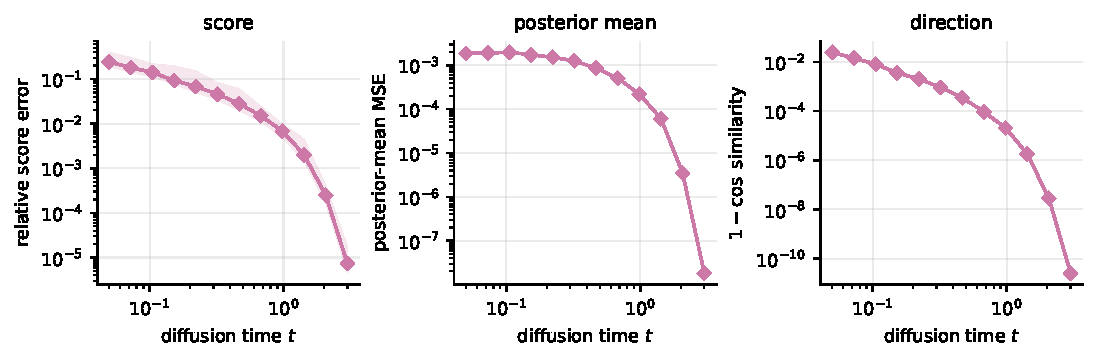
\includegraphics[width=0.86\textwidth]{fig_closure_vs_t.pdf}
\caption{What the Gaussian second-order baseline costs, against sum-product under the true kernel.
By Proposition~\ref{prop:lmmse} this gap is exactly the price of replacing the prior by its
covariance-matched Gaussian, so it measures non-Gaussianity rather than approximation quality.
Laplace chain, $\corr=0.85$; median over seeds with the $10$--$90$ percentile band.}
\label{fig:closure}
\end{figure}

\section{Learning the chain from noised sequences}

Now treat the kernel as unknown, observe only noised sequences $\vx^\mu$, and write
$\Lik(\params)=\sum_\mu\log P_{t,\params}(\vx^\mu)$. Gradient ascent on $\Lik$ looks expensive:
$\Lik$ is defined through the recursion, so differentiating it appears to need backpropagation
through $2(\nsites-1)$ message updates. It does not.

%% SHARED SECTION -- included by paper/main.tex and paper/workshop.tex.
%% Edit here, never in a copy. This file exists because the four documents
%% disagreeing with each other is the failure this rebuild was for.

\begin{proposition}[Exact gradient from one sum-product pass]
\label{prop:fisher}
With $\Xis$ the expected transition mass between grid points,
\begin{equation}
\label{eq:xi}
\Xis_{kl} \;=\; \sum_{\mu=1}^{\nseq}\sum_{i=2}^{\nsites}
P\!\left(a_{i-1}=\gridpt{k},\; a_i=\gridpt{l} \;\middle|\; \vx^\mu\right),
\end{equation}
the gradient of the \emph{marginal} log-likelihood is
\begin{equation}
\label{eq:fisher}
\nabla_\params \Lik(\params)
= \sum_{\mu}\E_\params\!\left[\nabla_\params \log P_\params(\va,\vx^\mu)\,\middle|\,\vx^\mu\right]
= \big\langle \Xis(\params),\; \nabla_\params \log \kernelth \big\rangle .
\end{equation}
\end{proposition}


\noindent
Sum-product is not a computation graph to backpropagate through; it supplies the conditional
expectation, and one forward--backward pass yields the exact gradient, verified against finite
differences of the discretised evidence to $\sim10^{-9}$. The statistic $\Xis$ is \emph{sufficient}
--- the complete-data log-likelihood is a sum over edges --- so maximisation never revisits the
data. For Gaussian innovations that maximisation is closed form, the belief-weighted Yule--Walker
equations, and gradient ascent and EM reach the same optimum; gradient ascent needs a tuned step
size and EM does not. We estimate the innovation as a mixture, so both the autoregressive
coefficient and the innovation density are free: twelve parameters at $\ncomp=4$.

\begin{remark}[Information asymmetry]
The estimator is given the Markov factorisation, the kernel's linear-autoregressive form, and
homogeneity across sites; the networks are given none of these. What follows measures the value of
that structure, not anything about neural denoisers in general.
\end{remark}

%% SHARED SECTION -- included by paper/main.tex and paper/workshop.tex.
%% Edit here, never in a copy. This file exists because the four documents
%% disagreeing with each other is the failure this rebuild was for.

\begin{table}[!htbp]
\caption{Relative denoising error against grid BP under the true kernel, averaged over the noise
schedule; sixteen seeds $\pm$ one standard error. The network's parameterisation is chosen on a
disjoint validation bundle, not the test set, and agrees with the test-set optimum in $99.4\%$ of
the $1{,}344$ cells. No crossing occurs in the range, so no data-equivalence factor is quoted.
\needsdata{EM budget: these ran at 120, the configured value is 400 (array 628943)}}
\label{tab:pointwise}
\centering
\begin{tabular}{rccc}
\toprule
sequences $\nseq$ & network & EM--BP ($12$ free) & ratio \\
\midrule
32   & $0.6613 \pm 0.0026$ & $\mathbf{0.0703 \pm 0.0051}$ & $9.4$ \\
64   & $0.5896 \pm 0.0029$ & $\mathbf{0.0541 \pm 0.0035}$ & $10.9$ \\
128  & $0.4942 \pm 0.0015$ & $\mathbf{0.0361 \pm 0.0024}$ & $13.7$ \\
256  & $0.3473 \pm 0.0012$ & $\mathbf{0.0259 \pm 0.0014}$ & $13.4$ \\
512  & $0.2359 \pm 0.0010$ & $\mathbf{0.0233 \pm 0.0010}$ & $10.1$ \\
1024 & $0.1685 \pm 0.0006$ & $\mathbf{0.0185 \pm 0.0011}$ & $9.1$ \\
2048 & $0.1364 \pm 0.0007$ & $\mathbf{0.0172 \pm 0.0008}$ & $7.9$ \\
\bottomrule
\end{tabular}
\end{table}


\noindent
Table~\ref{tab:pointwise} is the point of the paper in one number: a ratio between $8$ and $14$
across seven doublings of the training set, against networks trained by denoising score matching in
both standard parameterisations, with the parameterisation chosen on a disjoint validation split.
The network at the largest budget has not reached the error the estimator attains at the smallest.
Markov structure, when the data has it, is worth an order of magnitude in sample efficiency.

\section{When structure is invisible to the marginals}

A chain makes what is being learned visible in low-order statistics. It need not be. Consider a
point starting on a ring of radius ${\approx}1$ at a uniformly random angle, taking a rotating
random walk; one sample is a whole $T$-frame trajectory, and the rotation $\psi$ is drawn per
trajectory from an unknown $p(\psi)$:
%% SHARED SECTION -- included by paper/main.tex and paper/workshop.tex.
%% Edit here, never in a copy.

\begin{equation}
\label{eq:ring}
z_0 = r_0(\cos\theta_0,\sin\theta_0),\quad r_0\sim \rho\,e^{-(\rho-1)^2/2\lambda},\;\;
\theta_0\sim U[0,2\pi),
\qquad
z_{u+1} = R_\psi z_u + \sigma\eta_u .
\end{equation}
 The rotation is a \emph{gauge}:
$U_\psi=\mathrm{blockdiag}(R_{-u\psi})$ is orthogonal, commutes with the isotropic channel, and
maps the model onto $\psi=0$, so $P_t(\vx\mid\psi)=P_t^{0}(U_\psi\vx)$ is closed form at any $T$.

%% SHARED SECTION -- included by paper/main.tex and paper/workshop.tex.
%% Edit here, never in a copy. This file exists because the four documents
%% disagreeing with each other is the failure this rebuild was for.

\begin{theorem}[Marginal blindness]
\label{thm:blind}
For the model \eqref{eq:ring} with uniform initial phase, every single-frame marginal is
independent of $\psi$, at every noise level. Consequently a per-frame model carries exactly zero
information about the rotation.
\end{theorem}


\noindent
The proof is two lines: $R^{u-k}\eta_k\overset{d}{=}\eta_k$ by isotropy and
$R^{u}z_0\overset{d}{=}z_0$ by the uniform phase, so $z_u\overset{d}{=}z_0+\sigma\sqrt{u}\,\xi$,
in which $\psi$ does not appear. The marginal is not degenerate --- it is a visible, non-Gaussian
ring whose radius grows as $\sqrt{u}$. It is simply blind to the dynamics. Radii are not evidence.

This gives the theorem its own control. EM over $p(\psi)$ on the joint likelihood recovers the
rotation to $0.15^\circ$ at low noise, degrading to $7.1^\circ$ at $t=1.4$ as the channel destroys
the information. The same EM scored with per-frame marginals cannot move: its likelihood is
constant in $\psi$, so the responsibilities equal $p(\psi)$ and the update is the identity. Across
$1{,}344$ cells the blind arm's estimate moves $0.0000$ in total variation from its uniform
initialisation --- a machine-precision zero, which is what a theorem predicting exactly no
information requires.

\begin{figure}[!htbp]
\centering
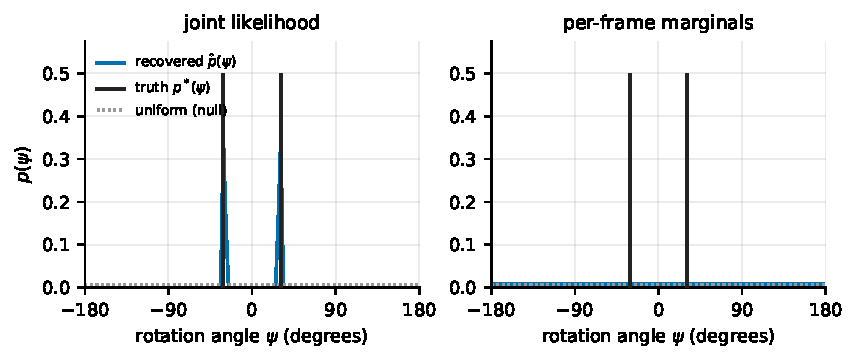
\includegraphics[width=0.60\textwidth]{fig_ring.pdf}
\caption{Recovered $p(\psi)$ against the two-species truth
$\tfrac12\delta_{+\omega}+\tfrac12\delta_{-\omega}$. Left: EM on the joint likelihood finds both
species. Right: the same run scored with per-frame marginals, which by Theorem~\ref{thm:blind}
cannot move off uniform, and does not. Shared $y$-axis.}
\label{fig:ring}
\end{figure}

\section{Scope, and what is open}

The estimator assumes exact first-order Markov structure; under a non-Markov prior it is
misspecified in a way more data does not repair, and the cost depends on which assumption breaks
--- a rank-one contamination a chain absorbs, long-range precision coupling it cannot represent.
Inference costs $O(\nsites\ngrid^{2})$ per sequence, well above a network forward pass, so the
advantage is in data and not wall-clock.

The open question is architectural. Sum-product on a chain suggests a network narrow but as deep
as twice the chain, unlike the tree-structured case where the natural depth is the tree's
\citep{mei2024unet,garnierbrun2024transformers}. Which architectures exploit Markovianity, and at
what depth, is what this setting is built to measure.

\bibliographystyle{unsrtnat}
\bibliography{references}

\clearpage
\appendix
\input{sections/workshop-appendix}

\end{document}
